\documentclass{article}
\usepackage[sexy, hdr, fancy]{evan}
\usepackage{graphicx}
\usepackage{float}
\graphicspath{.}
\setlength{\droptitle}{-4em}

\newcommand{\vwi}{{\bf w}_i}
\newcommand{\vw}{{\bf w}}
\newcommand{\vx}{{\bf x}}
\newcommand{\vy}{{\bf y}}
\newcommand{\vxi}{{\bf x}_i}
\newcommand{\yi}{y_i}
\newcommand{\vxj}{{\bf x}_j}
\newcommand{\vxn}{{\bf x}_n}
\newcommand{\yj}{y_j}
\newcommand{\ai}{\alpha_i}
\newcommand{\aj}{\alpha_j}
\newcommand{\X}{{\bf X}}
\newcommand{\Y}{{\bf Y}}
\newcommand{\vz}{{\bf z}}
\newcommand{\msigma}{{\bf \Sigma}}
\newcommand{\vmu}{{\bf \mu}}
\newcommand{\vmuk}{{\bf \mu}_k}
\newcommand{\msigmak}{{\bf \Sigma}_k}
\newcommand{\vmuj}{{\bf \mu}_j}
\newcommand{\msigmaj}{{\bf \Sigma}_j}
\newcommand{\pij}{\pi_j}
\newcommand{\pik}{\pi_k}
\newcommand{\D}{\mathcal{D}}
\newcommand{\el}{\mathcal{L}}
\newcommand{\N}{\mathcal{N}}
\newcommand{\vxij}{{\bf x}_{ij}}
\newcommand{\vt}{{\bf t}}
\newcommand{\yh}{\hat{y}}
\newcommand{\code}[1]{{\footnotesize \tt #1}}
\newcommand{\alphai}{\alpha_i}

\lhead{Homework 4}
\rhead{Machine Learning}
\lfoot{}
\cfoot{\thepage}

\begin{document}
\title{Homework 4}
\maketitle
\thispagestyle{fancy}


\section{Analytical (60 points)}

\paragraph{1) Clustering (14 points)}

We want to cluster the data set $\vx_1,\ldots,\vx_n$ using the K-means algorithm. The K-means algorithm partitions the $n$ observations into $k$ sets ($k < n$) $\mathbf{S} = \{S_1, S_2, \ldots, S_k\}$ so as to minimize the within-cluster sum of squares:
\begin{eqnarray*}
	\mathop{\textrm{argmin}}_{\mathbf{S}=\{S_1,\ldots,S_k\}}\sum_{j=1}^k\sum_{\vxi\in S_j}\|\vx_i-\mu_j\|_2^2
\end{eqnarray*}
where $\mu_j$ is the mean of the examples in $S_j$.

\begin{enumerate}[(a)]
	\item Prove that the objective is non-increasing after each E/M step.
		\begin{proof}
			Suppose at some EM step, we have $\theta=\left\{ \mu_1, \cdots, \mu_k \right\}$ is a vector containing the centroid values. Then $Z=\left\{ r_{nk} \right\}$ is a binary matrix where $r_{ij}=1$ if $x_i$ is in cluster $j,$ and 0 otherwise. Thus our objective function can be written as
			\begin{align*}
				J &= \sum_{i=1}^{n} \sum_{j=1}^{k} r_{ij} \left\lVert x_i-\mu_j \right\rVert_2^2
			\end{align*}
			Then using the update rules
			\begin{align*}
				r_{ij}^{new} &= \begin{cases}
					1 & j=\argmin_{\ell} \left\lVert x_i-\mu_\ell \right\rVert_2^2 \\
					0 & \text{otherwise}
				\end{cases}
			\end{align*}
			we have that
			\begin{align*}
				\sum_{j=1}^{k} r_{ij}^{new} \left\lVert x_i-\mu_j \right\rVert_2^2 &= \min_j \left\lVert x_i-\mu_j \right\rVert_2^2 \le \left\lVert x_i-\mu_\ell \right\rVert_2^2, \quad \forall \ell
			\end{align*}
			and thus since $\sum_{j=1}^{k} r_{ij}\left\lVert x_i-\mu_j \right\rVert_2^2 = \left\lVert x_i-\mu_\ell \right\rVert$ for some $\ell,$ we have
			\begin{align*}
				\sum_{i=1}^{n} \sum_{j=1}^{k} r_{ij}^{new}\left\lVert x_i-\mu_j \right\rVert_2^2\le \sum_{i=1}^{n} \sum_{j=1}^{k} r_{ij}\left\lVert x_i-\mu_j \right\rVert_2^2
			\end{align*}
			so the objective is non-increasing after each E step. Next, using the update rule
			\begin{align*}
				\mu_j^{new} &= \frac{\sum_{i}^{}r_{ij}^{new} x_i}{\sum_{i}^{}r_{ij}^{new}}
			\end{align*}
			we have the objective (after switching order of summation)
			\begin{align*}
				\sum_{i=1}^{n} \sum_{j=1}^{k} r_{ij}^{new} \left\lVert x_i-\mu_j^{new} \right\rVert_2^2 = \sum_{j=1}^{k} \sum_{i=1}^{n} r_{ij}^{new} \left\lVert x_i-\mu_j^{new} \right\rVert_2^2 = \sum_{j=1}^{k} \sum_{ x_i\in S_j} \left\lVert x_i-\mu_j^{new} \right\rVert_2^2
			\end{align*}
			where $\mu_j^{new}=\mu(S_j)$ as defined. From the previous homework, we know that $\mu(S_j)$ minimizes the sum of squared errors, so
			\begin{align*}
				\sum_{i=1}^{n} r_{ij}^{new} \left\lVert x_i-\mu_j^{new} \right\rVert=\sum_{x_i\in S_j}^{}\left\lVert x_i-\mu_j^{new} \right\rVert_2^2\le \sum_{x_i\in S_j}^{} \left\lVert x_i-\mu_j \right\rVert_2^2 = \sum_{i=1}^{n} r_{ij}^{new}\left\lVert x_i-\mu_j \right\rVert_2^2
			\end{align*}
			and thus
			\begin{align*}
				\sum_{j=1}^{k} \sum_{x_i\in S_j}^{} \left\lVert x_i-\mu_j^{new} \right\rVert_2^2= \sum_{j=1}^{k} \sum_{i=1}^{n} r_{ij}^{new} \left\lVert x_i-\mu_j^{new} \right\rVert &\le \sum_{j=1}^{k} \sum_{i=1}^{n} r_{ij}^{new} \left\lVert x_i-\mu_j \right\rVert_2^2
			\end{align*}
		\end{proof}

	\item One variant is called K-medoids. K-medoids is similar to K-means: both K-means and K-medoids minimize the squared error. However, unlike K-means, K-medoids chooses a training example as a cluster center (medoid). It is more robust to noise and outliers as compared to k-means because it minimizes a sum of pairwise dissimilarities instead of a sum of squared Euclidean distances. 

		Give an example to illustrate that K-medoids will be more robust to outliers than K-means.
		\begin{answer*}
			Consider the dataset $\left\{ 1, 2, 3, 4, 1000 \right\}$ with 1 cluster. Then under K-means, the center is at $\frac{1+2+3+4+1000}{5}=202,$ but under K-medoids, the center is at 3. Thus K-medoids is more robust to outliers because 3 is a better approximation for the cluster center than 202 is.
		\end{answer*}

	\item Another variant of K-means is to change the distance metric to the L1 distance, which is more robust to outliers. In this case, we are minimizing:
		\begin{align}
			\min_{S=\{S_1,...,S_k\}}\sum_{j=1}^k\sum_{\vxi\in S_j}\|\vx_j-\mu_j\|_1
		\end{align}
		where $\mu_j$ is the center of $S_j$ w.r.t. to L1 distance. It turns out that computing the medians is involved when computing the cluster center. That is why this algorithm is call K-medians. Does the cluster center have to be an actual instance from the dataset? Explain why.
		\begin{answer*}
			The median does not need to be an actual instance from the dataset. If there were an even number of points, then the median would be the average between the two "middle" points, which might not be in the dataset.
		\end{answer*}
\end{enumerate}

\newpage
\paragraph{2) Expectation-Maximization (12 points)} 

As we discussed in class, clustering objectives are non-convex. Therefore, different initializations will lead to different clustering solutions.

As an example, take Gaussian mixture model (GMM) clustering. Suppose all the parameters of the GMM are initialized such that all components/clusters have the same mean $\mu_k=\hat{\mu}$ and same covariance $\Sigma_k=\hat{\Sigma}$ for all $k=1,\ldots,K$.
\begin{enumerate}[(a)]
	\item Prove that the EM
		algorithm will converge after a single iteration for any choice of the initial mixing coefficients $\pi$.
		\begin{proof}
			In the E step, using the fact that $\mu_k=\hat\mu$ and $\Sigma_k=\hat\Sigma$ for all $k,$ we have
			\begin{align*}
				\gamma(z_{nk}) &= \frac{\pi_k \mathcal N\left(x_n\mid \mu_k, \Sigma_k\right)}{\sum_{j=1}^{K}\pi_j \mathcal N\left( x_n\mid \mu_k, \Sigma_k \right)} = \frac{\pi_k \mathcal N\left( x_n\mid \hat\mu, \hat\Sigma \right)}{\sum_{j=1}^{K} \pi_j \mathcal N\left( x_n\mid \hat\mu, \hat\Sigma \right)} = \frac{\pi_k}{\sum_{j=1}^{K}\pi_j} = \pi_k
			\end{align*}

			Then in the M step, we have
			\begin{align*}
				N_k &= \sum_{n=1}^{N} \gamma(z_{nk}) = \sum_{n=1}^{N} \pi_k = N\pi_k \\
				\implies \mu_k^{new} &= \frac{1}{N_k} \sum_{n=1}^{N} \gamma(z_{nk}) x_n = \frac{1}{N\pi_k} \sum_{n=1}^{N} \pi_k x_n = \frac{1}{N} \sum_{n=1}^{N} x_n = \bar x \\
				\implies\Sigma_k^{new} &= \frac{1}{N_k} \sum_{n=1}^{N} \gamma(z_{nk}) \left( x_n-\mu_k^{new} \right)\left( x_n-\mu_k^{new} \right)^T = \frac{1}{N\pi_k} \sum_{n=1}^{N} \pi_k \left( x_n- \bar x\right) \left( x_n-\bar x \right)^T \\
				&= \frac{1}{N} \sum_{n=1}^{N} \left( x-\bar x \right)\left( x-\bar x \right)^T = \Sigma \\
				\implies \pi_k^{new} &= \frac{N_k}{N} = \frac{N\pi_k}{N} = \pi_k
			\end{align*}

			Now, we are in the exact same situation as the initialization, where both means and covariances are equal for all $k$ since $\mu_k=\bar x$ and $\Sigma_k=\Sigma.$ Thus, if we were to perform another EM step, we would find that the parameters $\mu_k^{new} = \bar x, \Sigma_k^{new}=\Sigma$ and $\pi_k^{new} = \pi_k.$ Thus since $\pi$ was arbitrary, the algorithm will have converged after a single iteration.
		\end{proof}

	\item Show that this solution has the property $\mu_k=\frac{1}{N}\sum_{n=1}^{N}\mathbf{x}_n$ and $\Sigma_k=\frac{1}{N}\sum_{n=1}^{N}(\mathbf{x}_n-\mu_k)(\mathbf{x}_n-\mu_k)^T$, where $N$ is the total number of examples. Note that this represents a degenerate case of the mixture model in which all of the components are identical, and in practice we try to avoid such solutions by using an appropriate initialization.
		\begin{proof}
			From part (a), at convergence of the EM algorithm, we have
			\begin{align*}
				\mu_k &= \frac{1}{N}\sum_{n=1}^{N} x_n, \quad\quad \Sigma_k = \frac{1}{N} \sum_{n=1}^{N} \left( x_n-\mu_k \right)\left( x_n-\mu_k \right)^T
			\end{align*}
		\end{proof}

\end{enumerate}

\newpage
\paragraph{3) Dimensionality Reduction (9 points)}

Show that in the limit $\sigma^2 \rightarrow 0$, the posterior mean~\eqref{eq:ppca_postmean}~\eqref{eq:ppca_mmtx} for the probabilistic PCA model becomes an orthogonal projection onto the principal subspace, as in conventional PCA~\eqref{eq:pca_result}.

\begin{align}
\mathbb{E}[\mathbf{z}\vert\mathbf{x}] &= \mathbf{M}^{-1}\mathbf{W}_{\mathrm{ML}}^{\mathrm{T}} (\mathbf{x} - \bar{\mathbf{x}})
\label{eq:ppca_postmean} \\
\mathbf{M} &= \mathbf{W}^{\mathrm{T}} \mathbf{W} + \sigma^2 \mathbf{I}
\label{eq:ppca_mmtx} \\
\mathbf{y} &= \mathbf{L}^{-1/2} \mathbf{U}^{\mathrm{T}} (\mathbf{x} - \bar{\mathbf{x}})
\label{eq:pca_result}
\end{align}
	
\begin{proof}
	We have
	\begin{align*}
		E\left[ z\mid x \right] = M\inv W_{ML}^T(x-\bar x) = (W^TW+\sigma^2I)\inv \left[ U\left(L-\sigma^2 I\right)^{1/2} R \right]^T(x-\bar x)
	\end{align*}
	In the limit as $\sigma^2\to 0,$ this becomes
	\begin{align*}
		E\left[ z\mid x \right] &= \left( W^TW \right)\inv \left( U L^{1/2} R \right)^T(x-\bar x) = (W^TW)\inv \left( R^T L^{1/2} U^T \right)(x-\bar x) \\
		&= \left( W^TW \right)\inv R\inv L^{1/2} U^T(x-\bar x) = \left( RW^TW \right)\inv L^{1/2} U^T(x-\bar x)
	\end{align*}
	where we have used the fact that $L$ is diagonal and $R$ is orthogonal, so $R^T=R\inv.$ Now $RW^TW=L,$ so we finally get
	\begin{align*}
		E\left[ z\mid x \right] = L\inv L^{1/2} U^T(x-\bar x) = L^{-1/2}U^T (x-\bar x) = y
	\end{align*}
\end{proof}


\newpage
\paragraph{4) Probabilistic PCA (10 points)}

Draw a directed probabilistic graphical model representing a discrete mixture of probabilistic PCA models in which each PCA model has its own values of $\mathbf{W}$, $\boldsymbol{\mu}$, and $\sigma^2$. Then draw a modified graph in which these parameter values are shared between the components of the mixture. The graph should represent the model for a single data point $\mathbf{x}$. (Hint: refer to slide 24 of the Dimensionality Reduction lecture as a starting point.)
\begin{soln}
	The graphical models are shown below using plate notation.
	\begin{figure}[ht]
		\centering
		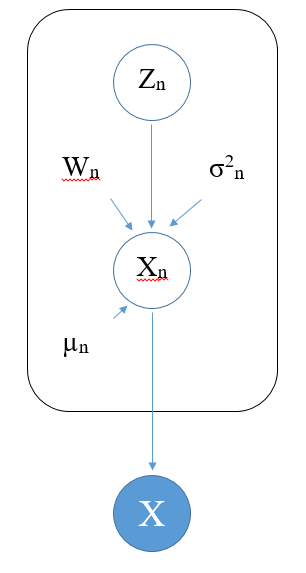
\includegraphics[width=4cm]{4a.PNG}
		\caption{Each PCA model has its own parameters}
	\end{figure}
	\begin{figure}[H]
		\centering
		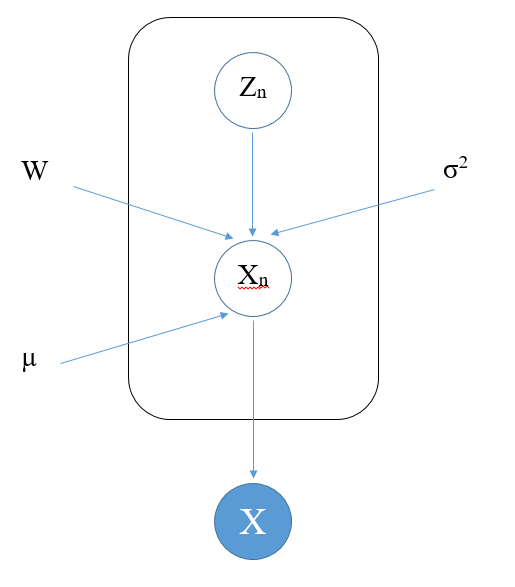
\includegraphics[width=7cm]{4b.PNG}
		\caption{Each PCA shares the parameters}
	\end{figure}	
\end{soln}


\newpage
\paragraph{5) Graphical Models (15 points)}

Consider the Bayesian Network given in Figure \ref{fig:bn}. Are the sets ${\bf A}$ and ${\bf B}$ d-separated given set ${\bf C}$ for each of the following definitions of ${\bf A}$, ${\bf B}$ and ${\bf C}$? Justify each answer.
\begin{figure}[h]
	\begin{center}
		\begin{tikzpicture}[style=thick,scale=1] 
			\newcommand{\nsize}{.8}
			\begin{scope}[shape=circle,minimum size=0.2cm] 
				\tikzstyle{every node}=[draw,fill] 
				\node[fill=none,scale=\nsize] (X_0) at (-2,2) {$\mathbf{X_0}$};
				\node[fill=none,scale=\nsize] (X_1) at (0,2) {$\mathbf{X_1}$};
				\node[fill=none,scale=\nsize] (X_2) at (2,2) {$\mathbf{X_2}$};
				\node[fill=none,scale=\nsize] (X_3) at (4,2) {$\mathbf{X_3}$};
				\node[fill=none,scale=\nsize] (X_4) at (1,1) {$\mathbf{X_4}$};
				\node[fill=none,scale=\nsize] (X_5) at (3,1) {$\mathbf{X_5}$};
				\node[fill=none,scale=\nsize] (X_6) at (0,0) {$\mathbf{X_6}$};
				\node[fill=none,scale=\nsize] (X_7) at (2,0) {$\mathbf{X_7}$};
				\node[fill=none,scale=\nsize] (X_8) at (4,0) {$\mathbf{X_8}$};
				\node[fill=none,scale=\nsize] (X_9) at (6,0) {$\mathbf{X_9}$};
				\draw [->] (X_0) -- (X_1);
				\draw [->] (X_2) -- (X_1);
				\draw [->] (X_3) -- (X_2);
				\draw [->] (X_2) -- (X_4);
				\draw [->] (X_2) -- (X_5);
				\draw [->] (X_4) -- (X_7);
				\draw [->] (X_5) -- (X_7);
				\draw [->] (X_6) -- (X_7);
				\draw [->] (X_7) -- (X_8);
				\draw [->] (X_9) -- (X_8);
			\end{scope} 
		\end{tikzpicture}
		\caption{A directed graph}
		\label{fig:bn}
	\end{center}
\end{figure}\\
\begin{enumerate}[a.]
	\item ${\bf A} = \{ X_3 \}$, ${\bf B} = \{ X_4 \}$, ${\bf C} = \{X_1,X_2\}$
		\begin{answer*}
			Yes. In the path $X_3\to X_2\to X_4,$ the arrows meet head to tail at $X_2\in C.$ In the path $X_3\to X_2\to X_5\to X_7\to X_4,$ the arrows meet head to tail at $X_2\in C.$ These are the only paths.

			If this was an MRF, then $A$ and $B$ would be d-separated because both paths pass through $X_2\in C.$
		\end{answer*}

	\item ${\bf A} = \{ X_5 \}$, ${\bf B} = \{X_4\}$, ${\bf C} = \{X_2,X_7\}$
		\begin{answer*}
			No. The path $X_5\to X_7\to X_4$ has arrows meeting head to head at $X_7\in C.$

			If this was an MRF, then $A$ and $B$ would be d-separated because the two possible paths are $X_5\to X_2\to X_4$ and $X_5\to X_7\to X_4,$ which pass through $X_2\in C$ and $X_7\in C,$ respectively.
		\end{answer*}

	\item ${\bf A} = \{X_4\}$, ${\bf B} = \{X_6\}$, ${\bf C} = \{X_8\}$
		\begin{answer*}
			No. The path $X_4\to X_7\to X_6$ has arrows meeting head to head at $X_7,$ which has descendent $X_8\in C.$

			If this was an MRF, then $A$ and $B$ would not be d-separated because there is no path from $X_4$ to $X_6$ passing through $X_8.$
		\end{answer*}

	\item ${\bf A} = \{X_5\}$, ${\bf B} = \{X_4\}$, ${\bf C} = \{X_2\}$
		\begin{answer*}
			Yes. In the path $X_5\to X_2\to X_4,$ the arrows meet tail to tail at $X_2\in C.$ In the path $X_5\to X_7\to X_4,$ the arrows meet head to head at $X_7,$ where $X_2$ is not a descendent.

			If this was an MRF, then $A$ and $B$ would not be d-separated because the path $X_5\to X_7\to X_4$ does not pass through any node in $C.$
		\end{answer*}

	\item ${\bf A} = \{X_6, X_9\}$, ${\bf B} = \{X_8\}$, ${\bf C} = \{X_3,X_1\}$
		\begin{answer*}
			No. The path $X_6\to X_7\to X_8$ has the arrows meet head to tail at $X_7\not\in C.$

			If this was an MRF, then $A$ and $B$ would not be d-separated because the path $X_6\to X_7\to X_8$ does not pass through any node in $C.$
		\end{answer*}
\end{enumerate}
Now assume that Figure 1 is a Markov Random Field, where each edge is undirected (just drop the direction of each edge.) Re-answer each of the above questions with justifications for your answers.


\end{document}
